\documentclass[problem]{mcs}

\begin{pcomments}
  \pcomment{FP_directed_graphs_and_probability} %\pcomment{from: S09.cp7r}
  \pcomment{prepared in Fall'11 for the final exam by S. Dwivedi}
  \pcomment{ARM edited 12/16/11}
\end{pcomments}

\pkeywords{
  digraphs
  DAGs
  probability
}

%%%%%%%%%%%%%%%%%%%%%%%%%%%%%%%%%%%%%%%%%%%%%%%%%%%%%%%%%%%%%%%%%%%%%
% Problem starts here
%%%%%%%%%%%%%%%%%%%%%%%%%%%%%%%%%%%%%%%%%%%%%%%%%%%%%%%%%%%%%%%%%%%%%

\newcommand{\Gdir}{\mathcal{G}_{\mbox dir}}

\begin{problem}
\bparts

\ppart For the directed acyclic graph (DAG) $\Gdir$ in
Figure~\ref{fig:Gdir}, a minimum-edge DAG with the same walk relation
can be obtained by removing some edges.  List these edges: \hfill
\examrule{1.5in}

\begin{figure}[here]
\begin{center}
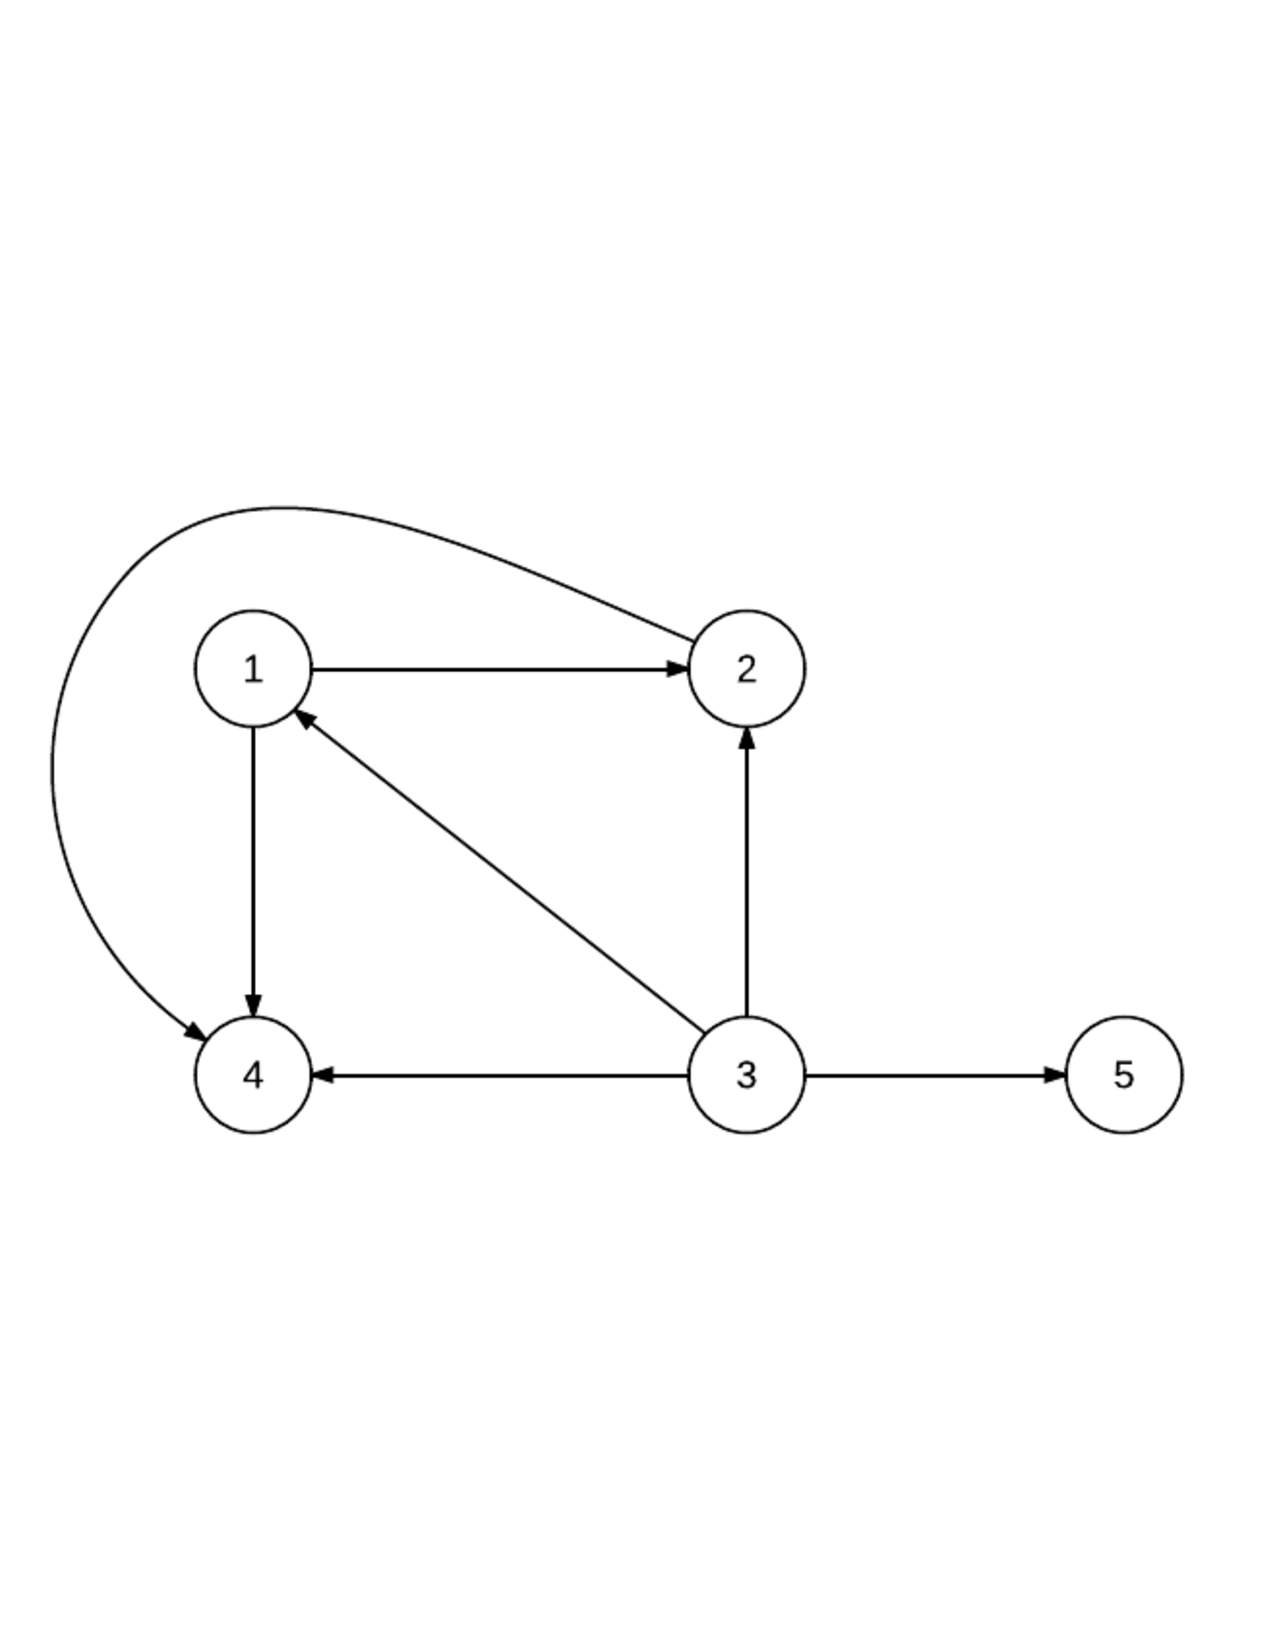
\includegraphics[scale=0.7]{dir_graph}
%\includegraphics[width=6in,height=7in]{mq1.jpg}
\end{center}
\caption{The DAG $\Gdir$}
\label{fig:Gdir}
\end{figure}

\begin{solution}
After removing edges $\diredge{3}{2}$ and $\diredge{3}{4}$, we get the
minimum DAG.
\end{solution}

\ppart List the vertices in a maximal antichain in $\Gdir$.\hfill \examrule{1.5in}

\begin{solution}
There are multiple maximal antichains. $\set{1,5}$, $\set{2,5}$,
$\set{4,5}$, etc.
\end{solution}
\eparts

Let $\mathcal{G}$ be the simple graph shown in Figure ~\ref{fig:simpleG}.

\begin{figure}[here]
\begin{center}
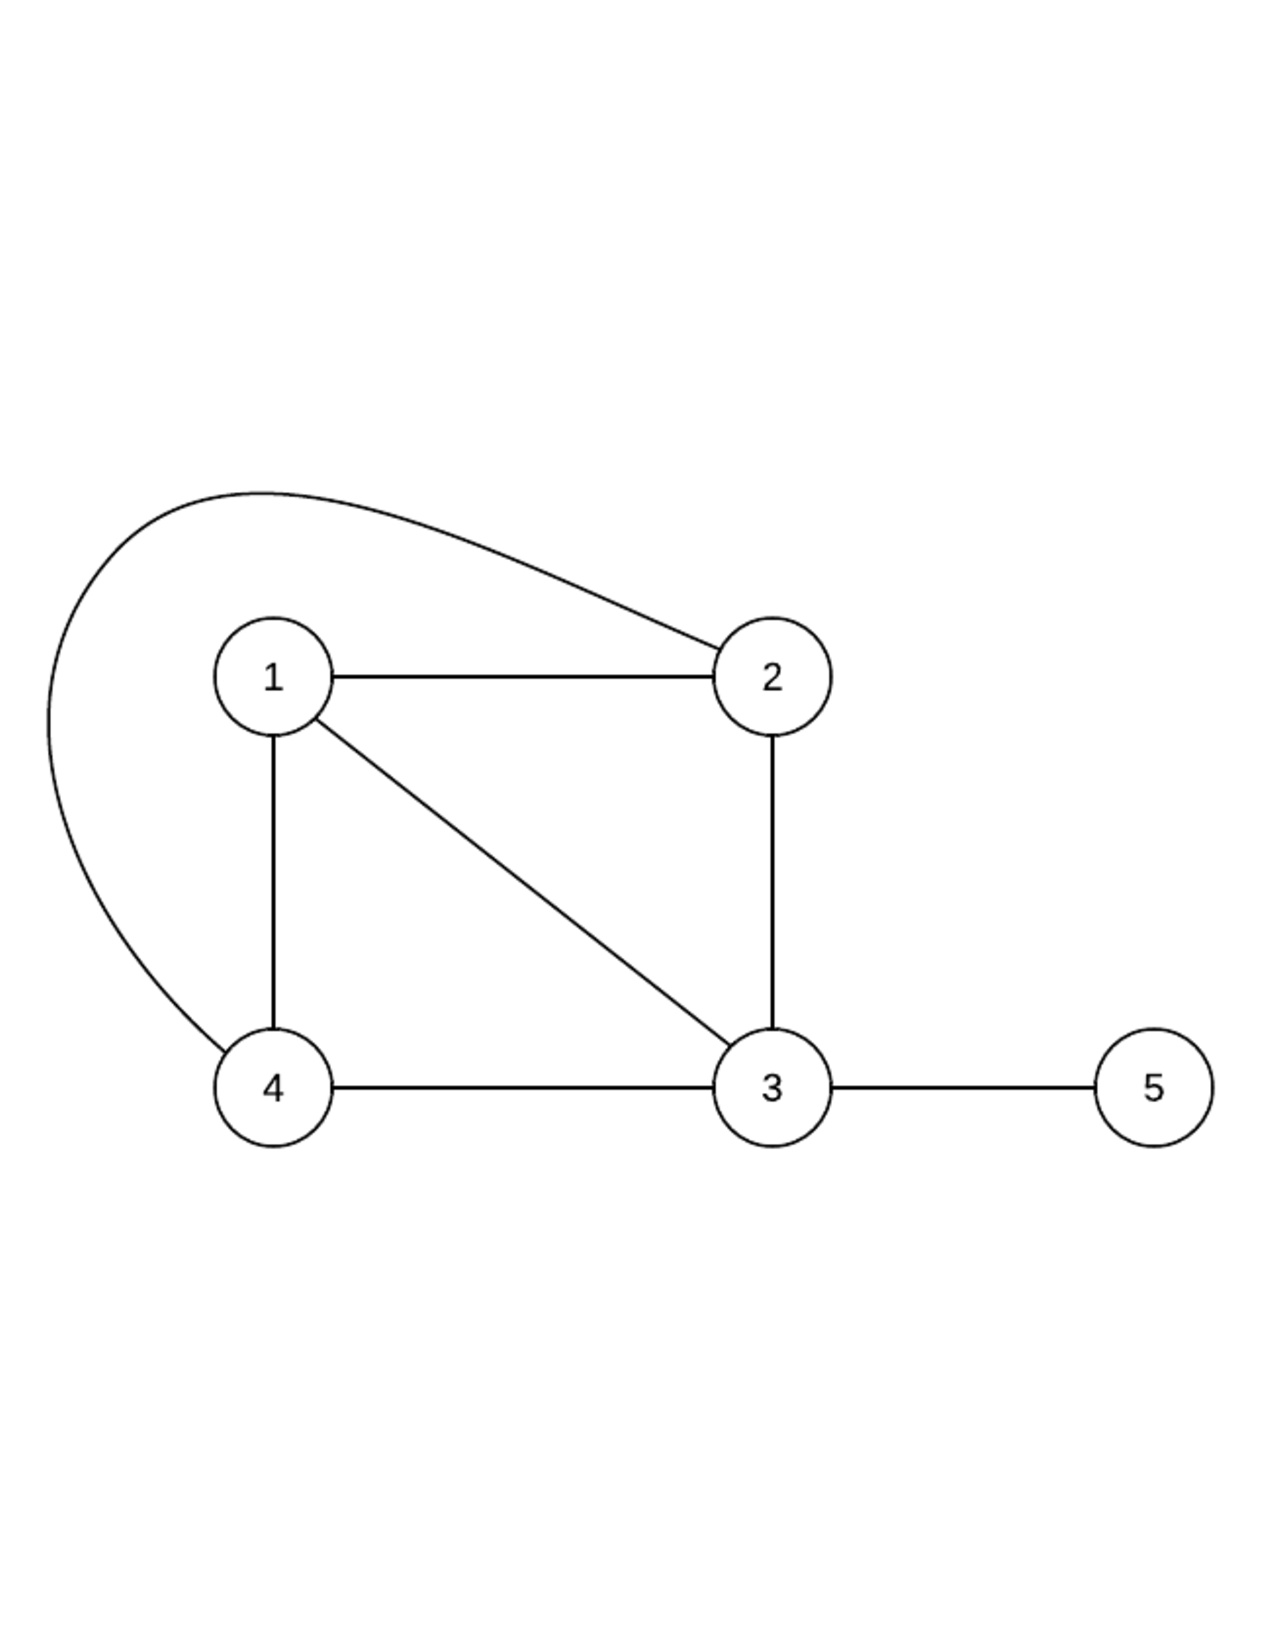
\includegraphics[scale=0.7]{simple_graph} 
%\includegraphics[width=6in,height=7in]{mq1.jpg}
\end{center}
\caption{Simple graph $\mathcal{G}$}
\label{fig:simpleG}
\end{figure}

A directed graph $D_\mathcal{G}$ can be randomly constructed from
$\mathcal{G}$ by choosing the direction of each directed edge
independently with equal likelihood.

\bparts

\pparts What is the probability that $D_\mathcal{G} = \Gdir$?\hfill \examrule

\begin{solution}
$2^{\card{\edges{\Gdir}}}$
\end{solution}

\eparts

Define the following events with respect to the random graph
$D_\mathcal{G}$:
\begin{align*}
T_1 \eqdef 123 \text{ is a directed cycle},\\
T_2 \eqdef 134 \text{ is a directed cycle},\\
T_3 \eqdef 124 \text{ is a directed cycle},\\
T_4 \eqdef 234 \text{ is a directed cycle}.
\end{align*}

\baprts
\ppart What is

$\pr{T_1}$? \hfill\examrule\\
$\pr{T_1 \intersect T_2}$? \hfill\examrule\\
$\pr{T_1 \intersect T_2 \intersect T_3}$? \hfill\examrule

\begin{solution}
\begin{align*}
\pr{T_1} = \frac{2}{2^3} & = \frac{1}{4}\\
\pr{T_1 \intersect T_2}  & = \frac{1}{16}\\
\pr{T_1 \intersect T_2 \intersect T_3}
                        & = 0.
\end{align*}
\end{solution}

\ppart What is the probability that $D_\mathcal{G}$ is a
DAG?\hfill\examrule.

\examspace{3in}

\begin{solution}
Using Inclusion-Exclusion principle,
\begin{align*}
\pr{\Gdir} \text{ is a DAG}}
   & = 1 - \pr{T_1 \union T_3 \union T_3 \union T_4}\\
   & = 1 - \sum_{i=1}^{4} \pr{T_i} + \sum_{i\neq j} \pr{T_i \intersect T_j} -
           \sum_{i\neq j \neq k} \pr{T_i \intersect T_j \intersect T_k} +
           \pr{T_1 \intersect T_2 \intersect T_3 \intersect T_4}\\
   & = 1 - 4 \cdot \frac{1}{4} + 6 \cdot \frac{1}{16} - 0+ 0\\
   & = \frac{3}{8}
\end{align*}

Observe that,
\begin{align*}
\pr{T_i \intersect T_j} = \frac{2}{2^5} & \text{ for $i \neq j$},\\
\pr{T_i \intersect T_j \intersect T_k} =0 & \text{for $i \neq j \neq k$, and}\\
\pr{T_1 \intersect T_2 \intersect T_3 \intersect T_4} = 0.
\end{align*}
\end{solution}

\eparts

\end{problem}

%%%%%%%%%%%%%%%%%%%%%%%%%%%%%%%%%%%%%%%%%%%%%%%%%%%%%%%%%%%%%%%%%%%%%
% Problem ends here
%%%%%%%%%%%%%%%%%%%%%%%%%%%%%%%%%%%%%%%%%%%%%%%%%%%%%%%%%%%%%%%%%%%%%

\endinput
